\chapter{\emph{Wiki} = Rápido}
\label{cha:wiki}

Esta reflexión escrita nació de notas, discusiones y lecturas entre fundadoras e integrantes de la organización. Aquí sistematizamos alrededor de cinco años de investigación de nuestro compromiso por transformar la forma de hacer política. En el texto se integran visiones desde y sobre Wikipolítica pero también sobre otros movimientos autónomos de vanguardia política, en diferentes latitudes y temporalidades.

Antes de comenzar, es preciso explicar qué es lo wiki y qué significa la wikipolítica. Wiki viene del hawaiano \emph{wiki wiki} que significa rápido. Es un concepto popular entre la comunidad del software libre para referirse a una visión colaborativa de la tecnología. Se popularizó gracias a Wikipedia, la enciclopedia libre. Fue usada por el programador Ward Cunningham a mediados del siglo pasado. Esta filosofía también está inspirada en actores como Aaron Schwartz, Richard Stallmann y de ella derivan proyectos de corte político pirata, como Library Genesis y Science Hub.\footnote{El manifiesto de estos dos proyectos se puede consultar en \url{custodians.online/spanish.html}.} Wikipolítica tuvo como precedente el Wikipartido. Surgió como algo parecido a un Partido pirata. \hlfix{Herederas}{¿por qué en femenino? hay que añadir una nota que lo explique} del \#YoSoy132, nos desarrollamos en una cultura de la colaboración, de la inteligencia colectiva y de visiones como el movimiento OPEN,\addref{} que busca fuentes o código, cultura y espacios abiertos. El mayor acierto desde nuestro punto de vistas fue considerar la tecnología como un componente central de la construcción contemporánea de lo político.

\begin{figure}[htbp]
	\centering
	
\includegraphics[scale=1]{wikipartido.png}
	\caption{Logo del Wikipartido en Jalisco}
	\label{fig:wikilogo}
\end{figure}

Fuimos influenciadas	 por las metodologías de diseño y negocios, como el \emph{Design thinking}, \emph{Scrum} o \emph{Agile}, y modelos de gobernanza participativa, como la sociocracia. Irónicamente, también aprendimos de las visiones locales como el \hlfix{municipalismo libertario}{sugiero resaltarlo} de Murray Bookchin\addref{} y reflexiones sobre el derecho a la ciudad.\addref{} Uno de los pilares comunicacionales de nuestra organización fue la política del encuentro. Desafortunadamente, la magnitud del problema de porqué la gente saldría a la calle a dialogar, cuando vive en la certidumbre del espectáculo (es decir, del deseo de consumir creado por los medios informativos), hace estériles todos nuestros esfuerzos por crear una posición política sobre cualquier cosa.

Según nuestros documentos oficiales,\addref{} nuestros principios incluyen democracia real y participativa, derechos humanos, localismo, rendición de cuentas, justicia social, innovación disruptiva, inteligencia colectiva, pedagogía política, apertura e inclusión y feminismo. Por otro lado, nuestros valores son honestidad, solidaridad, comunidad, deliberación, \hlfix{resiliencia}{Es un término de moda, pero ¿es necesario usarlo?} y sustentabilidad. Sin embargo, este marco ético tiene problemas importantes como establecer criterios para hacer interactuar los principios, porque su interpretación depende de la posición desde la cual se concibe el fenómeno político, o de las capacidades, de las motivaciones de quienes participan y de muchas otras cuestiones.

La construcción de este proyecto político ha sido señalada por intelectuales y personas de la crítica como un simulacro \hlfix{buena onda}{se debe resaltar esto en cursivas} del juego político partidista. Pese a reconocer que nuestra organización no habla desde conocimientos situados sino desde las abstracciones universalistas que caracteriza a la política tradicional de \emph{onvres}, no creemos que el \hlfix{buenaondismo}{Ibid.} de quienes tuvieron el mando informalmente fuera un gesto descuidado. Cada vez que alguien evadía la pregunta de en qué posición del espectro político nos encontrábamos, hacía una posición estratégica pero también intelectual, al hablar sobre una entidad política en formación que requiere responder ciertas cuestiones para poder presentarse públicamente a distintas audiencias que la legitiman. Muy probablemente se ha dicho poco sobre nuestras posiciones por la incapacidad de reconocer un hecho fundamental de toda política del futuro y ese hecho es que nuestras posiciones intelectuales son necesariamente estratégicas en la medida en que hasta el más mínimo pronunciamiento contiene en sí una visión del mundo que requiere ser justificada si quiere ser considerada como una alternativa seria.

Al titubeo público de nuestra fuerza política nosotras le decimos \emph{ciudadanismo radical} por plantear al ciudadano común como la subjetividad, como \enquote{la persona},\revquotes{} en disputa contra la partidocracia, \hlfix{un}{entendida como\ldots} conjunto de ratas corruptas cuya existencia supone la raíz de todos los problemas. Esta visión fue la predilecta entre varios hombres y algunas compañeras, por ser la ideal para justificar la pretensión de algunas personas para construir una plataforma política electoral, como lo hiciera Podemos después del 15M o movimiento de los indignados. El hambre poco disimulada de quienes lideraban se apoderó muy pronto de la organización aunque el Wikipartido, antecedente de la Wikipolítica, era un proyecto político un poco distinto a la grilla burda, era un proyecto de naturaleza \hlfix{radicalmente pirata}{¿y esto qué significa}.

\begin{figure}[htbp]
	\centering
	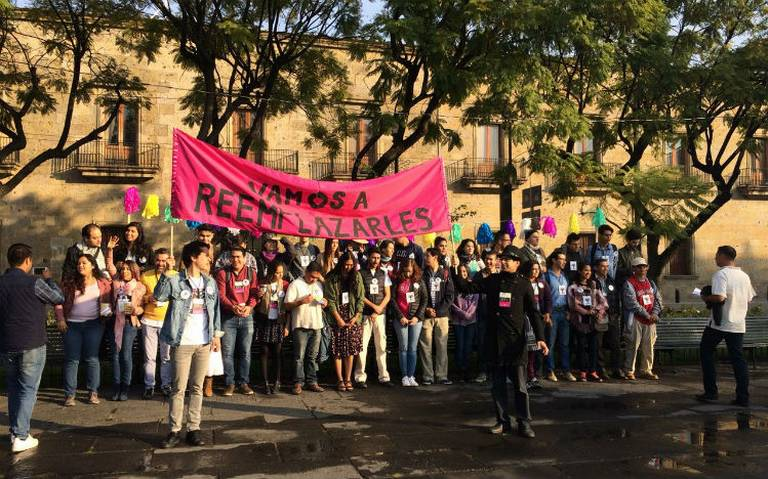
\includegraphics[width=\linewidth]{reemplazarles.jpg}
	\caption{¡Vamos a reemplazarles!}
	\label{fig:reemplazo}
\end{figure}

Para muchas de nosotras era inconcebible que un protopartido pirata se convirtiera en otro partido electorero aunque las personas que lo convirtieron en el fracaso electoral que fue, usaron diversas técnicas de la \hlfix{Ciencia Politica}{¿necesita las mayúsculas?} para conducir a toda la asamblea hacia su propio interés. El cambio de piratas a populistas se explica si pensamos que una organización es un juego con reglas formales e informales. En este caso, las personas más capaces decidieron renunciar a la consigna política que crearon, para usar el poder que les da pertenecer a una élite (familias poderosas, alta educación académica, carisma, estatura, capacidad para hablar, habilidades de negociación o de ciertas jergas populares y agendas consensadas en el movimiento \#YoSoy132) para perseguir su beneficio personal con una justificación mediática suficiente: \emph{somos las personas indignadas que se levantaron en México para denunciar todos los problemas y encontrar todas las soluciones.} Quizá muchas de estas personas ignoraban (y quizá todavía lo hacen) el aura de capital social que les rodea y que las hace prácticamente intocables frente al asedio de corporaciones económicas y partidistas, además de agencias de inteligencia que a lo largo de los últimos sesenta o setenta años se han dedicado a asediar e incluso asesinar a la oposición popular organizada (o sea a las organizaciones sin integrantes de abolengo) en México.

Para quienes nos posicionamos por la pregunta de cómo hacer efectiva y concreta esa otra forma de hacer política, lo primero que aprendimos fue 
\begin{enumerate}
	\item que en México toda forma política es corporativa y está programada en nuestra psique a un nivel \hlfix{casi}{queda mejor decir \emph{prácticamente}.} inconsciente, 
	\item a pensar en los problemas de responsabilidad individual como problemas que se pueden atacar cultivando nuestras potencias, fortaleciendo nuestras capacidades y reconociendo nuestras necesidades.
\end{enumerate}

No creemos en lo que mucha gente dice, que en México la gente es apática y apolítica. El espíritu agachado, arrabalero y huevón de que hablaba la filosofía ---priísta, por cierto--- del mexicano, y que todavía hoy constituye la ideología \emph{whitexican}, es en realidad la abnegación de sabernos sin las armas para combatir, de no querer que nuestras rebeliones no produzcan nada más que muertos y desaparecidos.

Sin embargo, a diferencia de hace unas décadas, hoy estamos en las condiciones tecnológicas para la conformación efectiva de un nuevo poder que cimbre el estado actual de las cosas. Para lograr una transformación real necesitamos accionar desde distintas aristas y facilitando la conexión estratégica entre distintos grupos políticos que buscan abrir y liberar flujos, que aumenten las potencias de las personas. La pregunta pedagógica es:

\begin{quote}
	¿cómo conciliamos todas estas cosas que hemos aprendido desde nuestra experiencia política con acciones articuladas y de gran escala, en diferentes niveles?\todo{Quizá valga la pena en una forma de destacar tipográficamente esto.}
\end{quote}

Hay que darnos cuenta, por ejemplo, de que el rencor contra la partidocracia puede venir inconscientemente de desear el derroche, el exceso y el poder que esa gente tiene. En ese sentido, es importante hacernos \hlfix{la pregunta}{son más de una pregunta, sugiero ponerlo en plural}: si estuviéramos en sus zapatos, ¿cómo crearíamos otras formas de poder? ¿Por qué desearíamos renunciar a nuestros privilegios? ¿Cómo vamos a crear una cultura del encuentro y no del consumo?

La construcción de esta organización política es una metáfora del diseño de una nueva configuración del Estado que permita encontrar un más allá a la catástrofe, que reina a escala micro, \hlfix{molecular}{¿por qué molecular?}, local, y macro, \hlfix{molar}{¿por qué molar?}, \hlfix{global}{¿no será mejor usar el término en español mundial en vez de este falso cognado del inglés?}. Es necesario pensar cómo lidiar con los intereses de actoras individuales, cómo vamos a desarrollar todas nuestras capacidades orientadas hacia un cambio multidimensional, desde dónde lo haremos y cómo conseguiremos recursos.

Estas necesidades se pueden sintetizar, por ejemplo, como infraestructura tecnológica, para innovar con las herramientas que conocemos, gestionadas por \hlfix{geeks}{En cursivas, por ser anglicismo.} por ejemplo; cartografías del poder a través de visualizaciones, organigramas y diagramas de flujo desarrollados por economistas, abogadas y disenadoras; y documentación sobre los protocolos que dan vida a una organización resiliente, a través de procesos y patrones de trabajo.

Así, este texto pretende dar algunas luces a la cuestión de la crisis y la catástrofe, delinear algunos juegos de ficción utópica y posibilidades para empezar a configurar esos territorios imposibles. Desarrollamos algunos síntomas de la crisis política contemporánea, proponemos un modelo para tratar de navegar entre los múltiples factores que causan la opresión de las formas de vida, tanto en su relación con los gobiernos como con sus propios cuerpos. Esta posición escritural es \textbf{La Partida} y podríamos bien señalarla como especulaciones estratégicas, como una corriente de la táctica política. La pregunta central que guiará nuestras reflexiones es \emph{cómo nos organizamos} para un más allá de la catástrofe, cómo creamos un nuevo horizonte. Para nosotras, la estrategia consiste en acciones para visibilizar y combatir las asimetrías de oportunidades y capacidades de las personas y la táctica en configurar prácticas y patrones para las operaciones concretas en el territorio y fuera de él, partiendo del reconocimiento de las circunstancias de cualquier persona que actúa, de cómo en ella se entrecruzan múltiples fuerzas de captura a distintas velocidades.